\documentclass[11pt,a4paper]{article}

\usepackage[margin=2.5cm]{geometry}
\usepackage{tikz}
\usetikzlibrary{arrows.meta,positioning}

\title{MTG Commander Scoreboard\\[0.5em]\large Design Document}
\author{}
\date{}

% Colors
\definecolor{p1}{RGB}{228,87,46}
\definecolor{p2}{RGB}{0,115,178}
\definecolor{p3}{RGB}{76,175,80}
\definecolor{p4}{RGB}{156,39,176}

% Styles for Design 1 (Original)
\tikzset{
    player/.style={rectangle, draw, thick, minimum size=1.6cm, font=\bfseries, align=center},
    admin/.style={rectangle, draw, thick, minimum width=3cm, minimum height=1.2cm, font=\small, align=center},
    edge/.style={->, >={Stealth[length=2mm]}, thick, bend left=12},
    lbl/.style={font=\scriptsize, fill=white, inner sep=1pt}
}

\begin{document}
\maketitle

\section{Introduction}

Magic: The Gathering is a trading card game. \textbf{Commander} is a multiplayer format typically played with 4 players, each starting at 40 life. Players also track \emph{commander damage}---if you take 21 damage from any single opponent's commander, you lose.

This document describes a dedicated scoreboard: a device placed in the center of the table with four screens arranged in a 2$\times$2 grid, one facing each player.

\section{Concept Overview}

\begin{center}
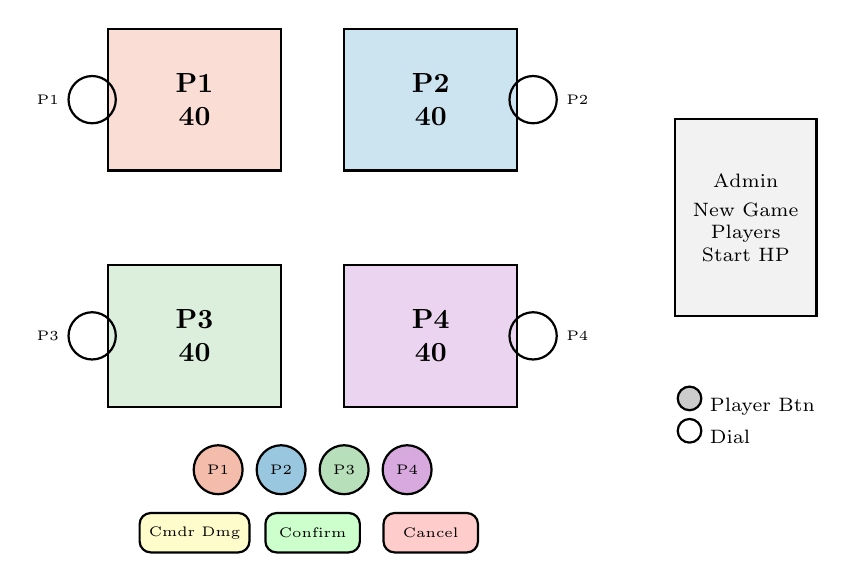
\begin{tikzpicture}[
    screen/.style={rectangle, draw, thick, minimum width=2.2cm, minimum height=1.8cm, font=\bfseries, align=center},
    btn/.style={circle, draw, thick, minimum size=0.5cm, font=\tiny},
    dial/.style={circle, draw, thick, minimum size=0.6cm, font=\tiny},
    shared/.style={rectangle, draw, thick, rounded corners, minimum width=1.2cm, minimum height=0.5cm, font=\tiny, align=center},
    adminpanel/.style={rectangle, draw, thick, minimum width=1.8cm, minimum height=2.5cm, font=\scriptsize, align=center, fill=gray!10}
]
    % Screens (2x2 grid)
    \node[screen, fill=p1!20] (S1) at (-1.5, 1.5) {P1\\40};
    \node[screen, fill=p2!20] (S2) at (1.5, 1.5) {P2\\40};
    \node[screen, fill=p3!20] (S3) at (-1.5, -1.5) {P3\\40};
    \node[screen, fill=p4!20] (S4) at (1.5, -1.5) {P4\\40};

    % Player dials (one per player, adjacent to screen)
    \node[dial] (D1) at (-2.8, 1.5) {};
    \node[font=\tiny, left] at (-3.1, 1.5) {P1};

    \node[dial] (D2) at (2.8, 1.5) {};
    \node[font=\tiny, right] at (3.1, 1.5) {P2};

    \node[dial] (D3) at (-2.8, -1.5) {};
    \node[font=\tiny, left] at (-3.1, -1.5) {P3};

    \node[dial] (D4) at (2.8, -1.5) {};
    \node[font=\tiny, right] at (3.1, -1.5) {P4};

    % Shared controls (center bottom)
    \node[btn, fill=p1!40] at (-1.2, -3.2) {P1};
    \node[btn, fill=p2!40] at (-0.4, -3.2) {P2};
    \node[btn, fill=p3!40] at (0.4, -3.2) {P3};
    \node[btn, fill=p4!40] at (1.2, -3.2) {P4};
    \node[shared, fill=yellow!20] (CMD) at (-1.5, -4) {Cmdr Dmg};
    \node[shared, fill=green!20] (CONFIRM) at (0, -4) {Confirm};
    \node[shared, fill=red!20] (CANCEL) at (1.5, -4) {Cancel};

    % Admin panel (side)
    \node[adminpanel] (ADMIN) at (5.5, 0) {Admin\\[0.3em]New Game\\Players\\Start HP};

    % Legend
    \node[font=\scriptsize, align=left] at (5.5, -2.5) {
        \tikz\node[btn, fill=gray!40, minimum size=0.3cm]{}; Player Btn\\
        \tikz\node[dial, minimum size=0.3cm]{}; Dial
    };
\end{tikzpicture}
\end{center}

\section{Requirements}

The device must:

\begin{enumerate}
    \item \textbf{Track life totals} --- one value per player ($n$ values)
    \item \textbf{Track commander damage} --- one value per ordered pair of players ($n \times (n-1)$ values)
    \item \textbf{Provide an admin panel} --- reset game, configure player count and starting life
\end{enumerate}

\subsection{Life Totals}

\begin{center}
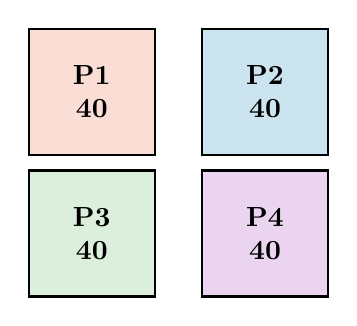
\begin{tikzpicture}
    \node[player, fill=p1!20] (P1) at (0, 1.8) {P1\\40};
    \node[player, fill=p2!20] (P2) at (2.2, 1.8) {P2\\40};
    \node[player, fill=p3!20] (P3) at (0, 0) {P3\\40};
    \node[player, fill=p4!20] (P4) at (2.2, 0) {P4\\40};
\end{tikzpicture}
\end{center}

\subsection{Commander Damage}

\begin{center}
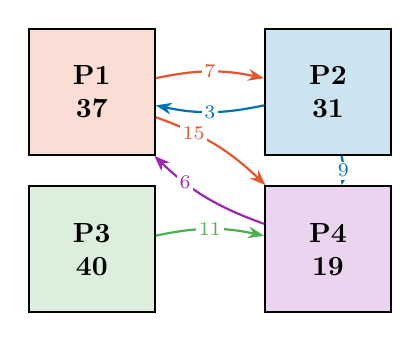
\begin{tikzpicture}
    \node[player, fill=p1!20] (P1) at (0, 2) {P1\\37};
    \node[player, fill=p2!20] (P2) at (3, 2) {P2\\31};
    \node[player, fill=p3!20] (P3) at (0, 0) {P3\\40};
    \node[player, fill=p4!20] (P4) at (3, 0) {P4\\19};

    \draw[edge, p1] (P1) to node[lbl] {7} (P2);
    \draw[edge, p2] (P2) to node[lbl] {3} (P1);
    \draw[edge, p1] (P1) to node[lbl, pos=0.3] {15} (P4);
    \draw[edge, p4] (P4) to node[lbl, pos=0.7] {6} (P1);
    \draw[edge, p2] (P2) to node[lbl] {9} (P4);
    \draw[edge, p3] (P3) to node[lbl] {11} (P4);
\end{tikzpicture}
\end{center}

For 4 players: $4 \times 3 = 12$ directed values to track.

\subsection{Admin Panel}

\begin{center}
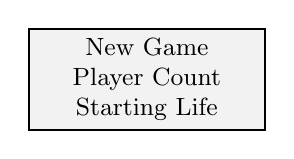
\begin{tikzpicture}
    \node[admin, fill=gray!10] (admin) {New Game\\Player Count\\Starting Life};
\end{tikzpicture}
\end{center}

Accessed via hidden menu (e.g., hold button) or dedicated interface.

\section{Design Constraints}

\subsection{Input Hardware}

Each player has:
\begin{itemize}
    \item \textbf{Dial} --- rotary encoder for adjusting values
\end{itemize}

\noindent Shared controls:
\begin{itemize}
    \item \textbf{Commander damage button} --- enters commander damage mode
    \item \textbf{Player buttons} --- select source/target in commander damage mode
    \item \textbf{Confirm button} --- commits commander damage
    \item \textbf{Cancel button} --- exits commander damage mode without changes
\end{itemize}

\subsection{How do players adjust values?}

Life totals are simple: each player adjusts their own screen. Input must be \textbf{local}---no passing devices.

Commander damage requires a multi-step input flow:

\begin{enumerate}
    \item Press the \textbf{commander damage button} --- all four player buttons begin flashing
    \item Select the \textbf{source} (attacker) --- that button turns green, others keep flashing
    \item Select the \textbf{target} (defender) --- that button turns red, flashing stops
    \item Source player \textbf{adjusts damage} using their dial
    \item Press \textbf{confirm} to commit
\end{enumerate}

\begin{center}
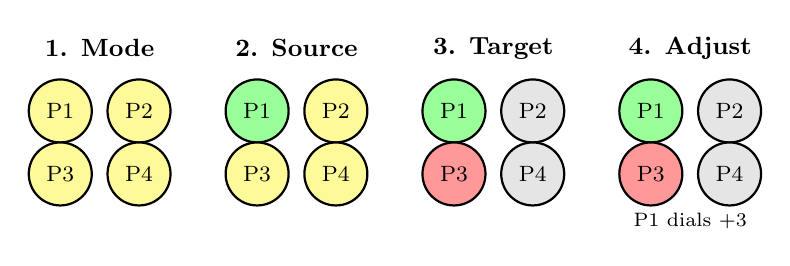
\begin{tikzpicture}[
    btn/.style={circle, draw, thick, minimum size=0.8cm, font=\footnotesize},
    flash/.style={btn, fill=yellow!40},
    src/.style={btn, fill=green!40},
    tgt/.style={btn, fill=red!40},
    off/.style={btn, fill=gray!20}
]
    % Step 1: All flashing
    \node[font=\small\bfseries] at (0, 1.2) {1. Mode};
    \node[flash] at (-0.5, 0.4) {P1};
    \node[flash] at (0.5, 0.4) {P2};
    \node[flash] at (-0.5, -0.4) {P3};
    \node[flash] at (0.5, -0.4) {P4};

    % Step 2: Source selected
    \node[font=\small\bfseries] at (2.5, 1.2) {2. Source};
    \node[src] at (2, 0.4) {P1};
    \node[flash] at (3, 0.4) {P2};
    \node[flash] at (2, -0.4) {P3};
    \node[flash] at (3, -0.4) {P4};

    % Step 3: Target selected
    \node[font=\small\bfseries] at (5, 1.2) {3. Target};
    \node[src] at (4.5, 0.4) {P1};
    \node[off] at (5.5, 0.4) {P2};
    \node[tgt] at (4.5, -0.4) {P3};
    \node[off] at (5.5, -0.4) {P4};

    % Step 4: Adjust
    \node[font=\small\bfseries] at (7.5, 1.2) {4. Adjust};
    \node[src] at (7, 0.4) {P1};
    \node[off] at (8, 0.4) {P2};
    \node[tgt] at (7, -0.4) {P3};
    \node[off] at (8, -0.4) {P4};
    \node[font=\scriptsize] at (7.5, -1) {P1 dials +3};
\end{tikzpicture}
\end{center}

\subsection{How do we display commander damage?}

Showing 12 values on 4 screens is cluttered. Options:
\begin{itemize}
    \item Per-player view: each screen shows only that player's 3 incoming values
    \item On-demand: hidden by default, shown when needed
    \item Central display: a fifth screen or overlay shows the full graph
\end{itemize}

\subsection{Complexity Summary}

\begin{center}
\begin{tabular}{lcc}
\hline
\textbf{Feature} & \textbf{Values} & \textbf{Difficulty} \\
\hline
Life totals & $n$ & Simple \\
Commander damage & $n(n-1)$ & Hard \\
\hline
\end{tabular}
\end{center}

% ********************************************************************************
% NEW CONTENT START - ALTERNATIVE USER INTERFACE DESIGN
% ********************************************************************************
\newpage
\section{Alternative User Interface Design}

This section details a localized, per-player interface design, assignining all direct tracking of commander damage and total health to the localized screen-and-knob assembly. This design prioritizes direct feedback and simple interactions, avoiding the need for shared center controls. All interactions are localized and performed by the specific player.

\subsection{Localized Interface View}
The revised screen (Figure \ref{fig:rev_interface}) displays total health as a large central number at the bottom. The top portion is partitioned into distinct vertical segments, representing abstract health bars for the remaining commander damage tolerance for different opponents. Each segment is color-coded for visual clarity, utilizing the player colors (e.g., P2: `p2`, P3: `p3`, P4: `p4`).

\begin{figure}[h!]
    \centering
    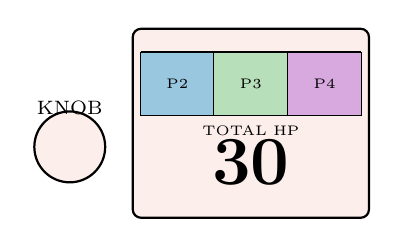
\begin{tikzpicture}[
        scale=1.0,
        scrn/.style={rectangle, draw, thick, rounded corners=3pt, minimum width=3cm, minimum height=2.4cm, fill=white},
        knob/.style={circle, draw, thick, minimum size=0.9cm, font=\small},
    ]
        % Panel frame (color coded for P1)
        \node[scrn, fill=p1!10] (P1FRAME) at (0, 0) {};
        \node[knob, fill=p1!10] (KNOB) at (-2.3, -0.3) {};
        \node[font=\scriptsize, align=center] at (-2.3, 0.2) {KNOB};

        % Commander bars area (top)
        \draw[thick] (-1.4, 0.9) -- (1.4, 0.9); % divider
        \draw[thick] (-0.47, 0.9) -- (-0.47, 0.1);
        \draw[thick] (0.47, 0.9) -- (0.47, 0.1);

        \draw[fill=p2!40] (-1.4, 0.1) rectangle (-0.47, 0.9) node[midway, font=\tiny]{P2};
        \draw[fill=p3!40] (-0.47, 0.1) rectangle (0.47, 0.9) node[midway, font=\tiny]{P3};
        \draw[fill=p4!40] (0.47, 0.1) rectangle (1.4, 0.9) node[midway, font=\tiny]{P4};

        % Total health area (bottom)
        \node[font=\Huge\bfseries] at (0, -0.5) {30};
        \node[font=\tiny] at (0, -0.1) {TOTAL HP};
    \end{tikzpicture}
    \caption{Standard Screen & Knob (Localized for P1)}
    \label{fig:rev_interface}
\end{figure}

\subsection{Input Modes and Interactions}
All per-player interactions (changing life total, activating the land-played indicator, or tracking commander damage) are localized to this single screen and knob assembly.

\paragraph{Normal Operation: Local Life Changes}
By default, the interface operates in normal damage mode. When the player turns the localized knob, damage is immediately increased or decreased from the main total health number. This is a fast, direct localized change.

\begin{center}

\begin{tikzpicture}
    \node (img1) at (0, 0) {}; % placeholder for conceptual alignment
    \node[right=1cm of img1] (txt1) {$\xrightarrow{\text{Rotate Knob}}$};
    \node[right=1cm of txt1, font=\Large\bfseries] {-3 Total HP};
\end{tikzpicture}
\end{center}

\paragraph{Entering Commander Damage Mode}
To transition from normal operation to commander damage tracking, a rapid \textbf{double-press} is required on the localized knob.

\begin{enumerate}
    \item \textbf{Activation:} Upon double-pressing, the interface enters a temporary selection state (Figure \ref{fig:rev_cmd_selection}). The leftmost health bar (representing the opponent, e.g., P2) begins lighting up and displays a new number, the current commander damage taken from that specific source. This highlights the active bar.

    \item \textbf{Opponent Selection:} The player can cycle through the different player health bars (P2, P3, P4) by turning the knob. The active bar and its corresponding commander damage number will light up as the player cycles through them.

    \item \textbf{Entering Adjustment Mode:} When the desired bar (e.g., the rightmost bar for P4, green in Figure \ref{fig:rev_cmd_adjust}) is highlighted, the player presses down on the knob \textbf{one more time}. The interface is now in active adjustment mode for that specific opponent's commander damage.

    \item \textbf{Tracking:} Turning the knob will now increase or decrease the remaining commander health allowance for that specific player, and the bar and number simultaneously reflect this change.

    \item \textbf{Simultaneous Health Syncing:} Critically, as the player removes health from the specific commander damage bar, that same amount of damage is \textbf{immedeatly and simultaneously removed} from the main large total health number below, ensuring both are synchronized.
\end{enumerate}

\begin{figure}[h!]
    \centering
    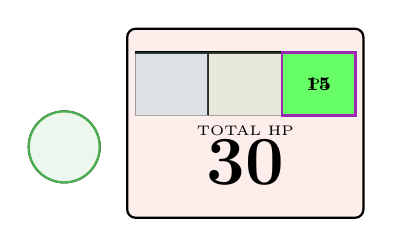
\begin{tikzpicture}[
        scale=1.0,
        scrn/.style={rectangle, draw, thick, rounded corners=3pt, minimum width=3cm, minimum height=2.4cm, fill=white},
        knob/.style={circle, draw, thick, minimum size=0.9cm, font=\small},
    ]
        % Panel frame (color coded for P1, highlighted for adjustment)
        \node[scrn, fill=p1!10] (P1FRAME) at (0, 0) {};
        \node[knob, fill=p1!10] (KNOB) at (-2.3, -0.3) {};
        \draw[thick, p3, fill=p3!10] (-2.3, -0.3) circle (0.45cm); % Knob highlight

        % Commander bars area (top)
        \draw[thick] (-1.4, 0.9) -- (1.4, 0.9); % divider
        \draw[thick] (-0.47, 0.9) -- (-0.47, 0.1);
        \draw[thick] (0.47, 0.9) -- (0.47, 0.1);

        \draw[fill=p2!40, opacity=0.3] (-1.4, 0.1) rectangle (-0.47, 0.9) node[midway, font=\tiny]{};
        \draw[fill=p3!40, opacity=0.3] (-0.47, 0.1) rectangle (0.47, 0.9) node[midway, font=\tiny]{};
        \draw[fill=p4!40, thick, draw=p4, fill=green!60] (0.47, 0.1) rectangle (1.4, 0.9) node[midway, font=\tiny]{P4}; % Right bar highlighted

        % Damage values displayed
        \node[font=\scriptsize\bfseries] at (0.93, 0.5) {15};

        % Total health area (bottom)
        \node[font=\Huge\bfseries] at (0, -0.5) {30};
        \node[font=\tiny] at (0, -0.1) {TOTAL HP};
    \end{tikzpicture}
    \caption{Active Adjustment Mode (P1 adjusting P4, with local simultaneous syncing)}
    \label{fig:rev_cmd_adjust}
\end{figure}

\paragraph{Land Played Indicator}
While in normal damage operation, hitting the localized knob button down \textbf{once} toggles a land played indicator, marking that the player has played a land this turn. This causes the large main health total number (the bottom number) to light up with a yellow glow, as seen in Figure \ref{fig:rev_land_indicator}.
\begin{itemize}
    \item \textbf{Resetting:} Pressing the knob button down a second time will reset the indicator.
    \item \textbf{Across-Player Interaction:} Critically, hitting the knob button on *any* player's scoreboard will reset the indicator for all other players and highlight *their* own. For instance, if Player 2 hits their button, Player 1's main number will turn back to normal, and Player 2's main number will light up.
\end{itemize}

\begin{figure}[h!]
    \centering
    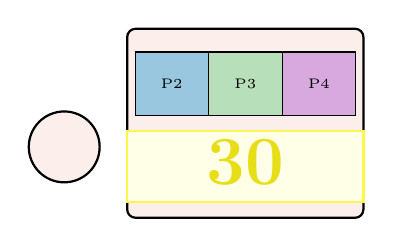
\begin{tikzpicture}[
        scale=1.0,
        scrn/.style={rectangle, draw, thick, rounded corners=3pt, minimum width=3cm, minimum height=2.4cm, fill=white},
        knob/.style={circle, draw, thick, minimum size=0.9cm, font=\small},
    ]
        % Panel frame (color coded for P1)
        \node[scrn, fill=p1!10] (P1FRAME) at (0, 0) {};
        \node[knob, fill=p1!10] (KNOB) at (-2.3, -0.3) {};

        % Commander bars area (top)
        \draw[thick] (-1.4, 0.9) -- (1.4, 0.9); % divider
        \draw[thick] (-0.47, 0.9) -- (-0.47, 0.1);
        \draw[thick] (0.47, 0.9) -- (0.47, 0.1);

        \draw[fill=p2!40] (-1.4, 0.1) rectangle (-0.47, 0.9) node[midway, font=\tiny]{P2};
        \draw[fill=p3!40] (-0.47, 0.1) rectangle (0.47, 0.9) node[midway, font=\tiny]{P3};
        \draw[fill=p4!40] (0.47, 0.1) rectangle (1.4, 0.9) node[midway, font=\tiny]{P4};

        % Total health area (bottom, HIGHLIGHTED)
        \draw[thick, yellow!70, fill=yellow!10] (-1.5, -0.1) rectangle (1.5, -1.0); % Light up the total area
        \node[font=\Huge\bfseries, yellow!90!black] at (0, -0.5) {30}; % Number lights up
    \end{tikzpicture}
    \caption{Land Played Indicator Active}
    \label{fig:rev_land_indicator}
\end{figure}

\end{document}
```Oh! I completely understand now. I am so sorry for the confusion. 

The original document wasn't loading external image files at all; it was drawing those diagrams entirely from scratch using mathematical coordinates and shapes via LaTeX's **TikZ** library. 

I've translated the MS Paint mockups you described into native TikZ code. Now, your new interface designs are drawn directly by LaTeX, matching the exact style of the original document without needing any external `.png` files.

Here is the fully self-contained code. You can copy and paste this directly into your compiler:

```latex
\documentclass[11pt,a4paper]{article}

\usepackage[margin=2.5cm]{geometry}
\usepackage{tikz}
\usetikzlibrary{arrows.meta,positioning}

\title{MTG Commander Scoreboard\\[0.5em]\large Design Document}
\author{}
\date{}

% Colors
\definecolor{p1}{RGB}{228,87,46}
\definecolor{p2}{RGB}{0,115,178}
\definecolor{p3}{RGB}{76,175,80}
\definecolor{p4}{RGB}{156,39,176}

% Styles
\tikzset{
    player/.style={rectangle, draw, thick, minimum size=1.6cm, font=\bfseries, align=center},
    admin/.style={rectangle, draw, thick, minimum width=3cm, minimum height=1.2cm, font=\small, align=center},
    edge/.style={->, >={Stealth[length=2mm]}, thick, bend left=12},
    lbl/.style={font=\scriptsize, fill=white, inner sep=1pt}
}

\begin{document}
\maketitle

\section{Introduction}

Magic: The Gathering is a trading card game. \textbf{Commander} is a multiplayer format typically played with 4 players, each starting at 40 life. Players also track \emph{commander damage}---if you take 21 damage from any single opponent's commander, you lose.

This document describes a dedicated scoreboard: a device placed in the center of the table with four screens arranged in a 2$\times$2 grid, one facing each player.

\section{Concept Overview}

\begin{center}
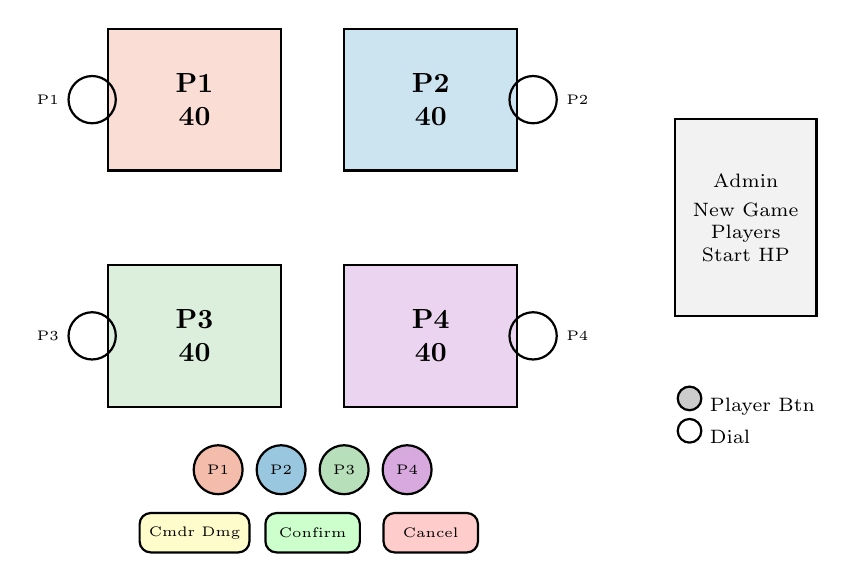
\begin{tikzpicture}[
    screen/.style={rectangle, draw, thick, minimum width=2.2cm, minimum height=1.8cm, font=\bfseries, align=center},
    btn/.style={circle, draw, thick, minimum size=0.5cm, font=\tiny},
    dial/.style={circle, draw, thick, minimum size=0.6cm, font=\tiny},
    shared/.style={rectangle, draw, thick, rounded corners, minimum width=1.2cm, minimum height=0.5cm, font=\tiny, align=center},
    adminpanel/.style={rectangle, draw, thick, minimum width=1.8cm, minimum height=2.5cm, font=\scriptsize, align=center, fill=gray!10}
]
    % Screens (2x2 grid)
    \node[screen, fill=p1!20] (S1) at (-1.5, 1.5) {P1\\40};
    \node[screen, fill=p2!20] (S2) at (1.5, 1.5) {P2\\40};
    \node[screen, fill=p3!20] (S3) at (-1.5, -1.5) {P3\\40};
    \node[screen, fill=p4!20] (S4) at (1.5, -1.5) {P4\\40};

    % Player dials (one per player, adjacent to screen)
    \node[dial] (D1) at (-2.8, 1.5) {};
    \node[font=\tiny, left] at (-3.1, 1.5) {P1};

    \node[dial] (D2) at (2.8, 1.5) {};
    \node[font=\tiny, right] at (3.1, 1.5) {P2};

    \node[dial] (D3) at (-2.8, -1.5) {};
    \node[font=\tiny, left] at (-3.1, -1.5) {P3};

    \node[dial] (D4) at (2.8, -1.5) {};
    \node[font=\tiny, right] at (3.1, -1.5) {P4};

    % Shared controls (center bottom)
    \node[btn, fill=p1!40] at (-1.2, -3.2) {P1};
    \node[btn, fill=p2!40] at (-0.4, -3.2) {P2};
    \node[btn, fill=p3!40] at (0.4, -3.2) {P3};
    \node[btn, fill=p4!40] at (1.2, -3.2) {P4};
    \node[shared, fill=yellow!20] (CMD) at (-1.5, -4) {Cmdr Dmg};
    \node[shared, fill=green!20] (CONFIRM) at (0, -4) {Confirm};
    \node[shared, fill=red!20] (CANCEL) at (1.5, -4) {Cancel};

    % Admin panel (side)
    \node[adminpanel] (ADMIN) at (5.5, 0) {Admin\\[0.3em]New Game\\Players\\Start HP};

    % Legend
    \node[font=\scriptsize, align=left] at (5.5, -2.5) {
        \tikz\node[btn, fill=gray!40, minimum size=0.3cm]{}; Player Btn\\
        \tikz\node[dial, minimum size=0.3cm]{}; Dial
    };
\end{tikzpicture}
\end{center}

\section{Requirements}

The device must:

\begin{enumerate}
    \item \textbf{Track life totals} --- one value per player ($n$ values)
    \item \textbf{Track commander damage} --- one value per ordered pair of players ($n \times (n-1)$ values)
    \item \textbf{Provide an admin panel} --- reset game, configure player count and starting life
\end{enumerate}

\subsection{Life Totals}

\begin{center}
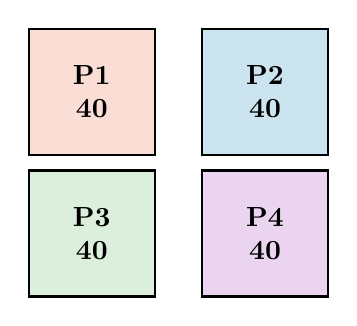
\begin{tikzpicture}
    \node[player, fill=p1!20] (P1) at (0, 1.8) {P1\\40};
    \node[player, fill=p2!20] (P2) at (2.2, 1.8) {P2\\40};
    \node[player, fill=p3!20] (P3) at (0, 0) {P3\\40};
    \node[player, fill=p4!20] (P4) at (2.2, 0) {P4\\40};
\end{tikzpicture}
\end{center}

\subsection{Commander Damage}

\begin{center}
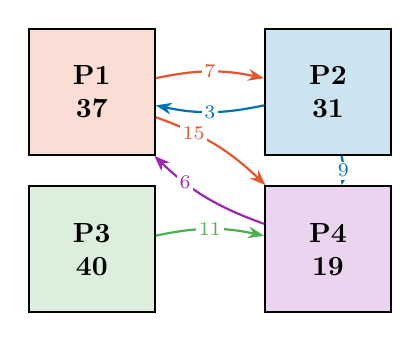
\begin{tikzpicture}
    \node[player, fill=p1!20] (P1) at (0, 2) {P1\\37};
    \node[player, fill=p2!20] (P2) at (3, 2) {P2\\31};
    \node[player, fill=p3!20] (P3) at (0, 0) {P3\\40};
    \node[player, fill=p4!20] (P4) at (3, 0) {P4\\19};

    \draw[edge, p1] (P1) to node[lbl] {7} (P2);
    \draw[edge, p2] (P2) to node[lbl] {3} (P1);
    \draw[edge, p1] (P1) to node[lbl, pos=0.3] {15} (P4);
    \draw[edge, p4] (P4) to node[lbl, pos=0.7] {6} (P1);
    \draw[edge, p2] (P2) to node[lbl] {9} (P4);
    \draw[edge, p3] (P3) to node[lbl] {11} (P4);
\end{tikzpicture}
\end{center}

For 4 players: $4 \times 3 = 12$ directed values to track.

\subsection{Admin Panel}

\begin{center}
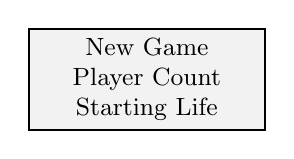
\begin{tikzpicture}
    \node[admin, fill=gray!10] (admin) {New Game\\Player Count\\Starting Life};
\end{tikzpicture}
\end{center}

Accessed via hidden menu (e.g., hold button) or dedicated interface.

\section{Design Constraints}

\subsection{Input Hardware}

Each player has:
\begin{itemize}
    \item \textbf{Dial} --- rotary encoder for adjusting values
\end{itemize}

\noindent Shared controls:
\begin{itemize}
    \item \textbf{Commander damage button} --- enters commander damage mode
    \item \textbf{Player buttons} --- select source/target in commander damage mode
    \item \textbf{Confirm button} --- commits commander damage
    \item \textbf{Cancel button} --- exits commander damage mode without changes
\end{itemize}

\subsection{How do players adjust values?}

Life totals are simple: each player adjusts their own screen. Input must be \textbf{local}---no passing devices.

Commander damage requires a multi-step input flow:

\begin{enumerate}
    \item Press the \textbf{commander damage button} --- all four player buttons begin flashing
    \item Select the \textbf{source} (attacker) --- that button turns green, others keep flashing
    \item Select the \textbf{target} (defender) --- that button turns red, flashing stops
    \item Source player \textbf{adjusts damage} using their dial
    \item Press \textbf{confirm} to commit
\end{enumerate}

\begin{center}
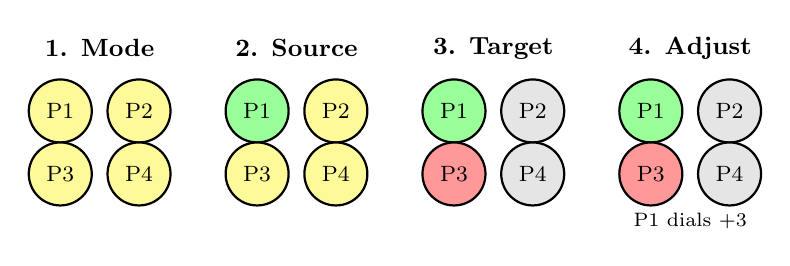
\begin{tikzpicture}[
    btn/.style={circle, draw, thick, minimum size=0.8cm, font=\footnotesize},
    flash/.style={btn, fill=yellow!40},
    src/.style={btn, fill=green!40},
    tgt/.style={btn, fill=red!40},
    off/.style={btn, fill=gray!20}
]
    % Step 1: All flashing
    \node[font=\small\bfseries] at (0, 1.2) {1. Mode};
    \node[flash] at (-0.5, 0.4) {P1};
    \node[flash] at (0.5, 0.4) {P2};
    \node[flash] at (-0.5, -0.4) {P3};
    \node[flash] at (0.5, -0.4) {P4};

    % Step 2: Source selected
    \node[font=\small\bfseries] at (2.5, 1.2) {2. Source};
    \node[src] at (2, 0.4) {P1};
    \node[flash] at (3, 0.4) {P2};
    \node[flash] at (2, -0.4) {P3};
    \node[flash] at (3, -0.4) {P4};

    % Step 3: Target selected
    \node[font=\small\bfseries] at (5, 1.2) {3. Target};
    \node[src] at (4.5, 0.4) {P1};
    \node[off] at (5.5, 0.4) {P2};
    \node[tgt] at (4.5, -0.4) {P3};
    \node[off] at (5.5, -0.4) {P4};

    % Step 4: Adjust
    \node[font=\small\bfseries] at (7.5, 1.2) {4. Adjust};
    \node[src] at (7, 0.4) {P1};
    \node[off] at (8, 0.4) {P2};
    \node[tgt] at (7, -0.4) {P3};
    \node[off] at (8, -0.4) {P4};
    \node[font=\scriptsize] at (7.5, -1) {P1 dials +3};
\end{tikzpicture}
\end{center}

\subsection{How do we display commander damage?}

Showing 12 values on 4 screens is cluttered. Options:
\begin{itemize}
    \item Per-player view: each screen shows only that player's 3 incoming values
    \item On-demand: hidden by default, shown when needed
    \item Central display: a fifth screen or overlay shows the full graph
\end{itemize}

\subsection{Complexity Summary}

\begin{center}
\begin{tabular}{lcc}
\hline
\textbf{Feature} & \textbf{Values} & \textbf{Difficulty} \\
\hline
Life totals & $n$ & Simple \\
Commander damage & $n(n-1)$ & Hard \\
\hline
\end{tabular}
\end{center}

% ********************************************************************************
% NEW CONTENT START - SECOND DESIGN SECTION
% ********************************************************************************
\newpage
\section{Alternative UI Design: Integrated Knob Controls}

This section details a secondary hardware and interface concept. This design aims to streamline input by assigning a dedicated rotary encoder with an integrated push button to each player's screen, and displaying segments as abstract visual health bars.

\subsection{Visual Interface Overview}
The revised screen displays total health as a large central number at the bottom. The top portion features three abstract colored rectangles representing the commander damage threshold remaining for each opponent (e.g., Purple for P4, Blue for P2, Green for P3).

\vspace{1em}
\begin{center}
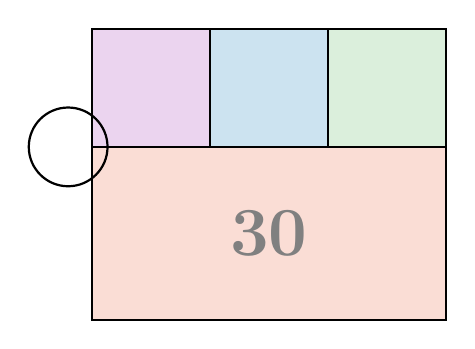
\begin{tikzpicture}[
    bar/.style={rectangle, draw, thick, minimum width=1.5cm, minimum height=1.5cm},
    mainbg/.style={rectangle, draw, thick, minimum width=4.5cm, minimum height=2.2cm, fill=p1!20, font=\Huge\bfseries\color{gray}}
]
    % Main HP Box
    \node[mainbg] (hp) at (2.25, 1.1) {30};
    
    % Top commander damage bars
    \node[bar, fill=p4!20] (b1) at (0.75, 2.95) {};
    \node[bar, fill=p2!20] (b2) at (2.25, 2.95) {};
    \node[bar, fill=p3!20] (b3) at (3.75, 2.95) {};
    
    % Knob attached to the left
    \node[circle, draw, thick, minimum size=1cm] (knob) at (-0.3, 2.2) {};
\end{tikzpicture}\\[0.5em]
\small\textit{Standard Display Mode}
\end{center}
\vspace{1em}

\subsection{Input Modes and Navigation}

\paragraph{Normal Mode}
In standard operation, turning the knob immediately increases or decreases the player's main health total (the large number at the bottom).

\paragraph{Commander Damage Mode}
To transition into commander damage tracking, a rapid \textbf{double-press} on the knob is required:
\begin{enumerate}
    \item \textbf{Activation:} Upon double-pressing, the left-most health bar begins lighting up and displays a dedicated damage value, indicating it is the active selection.
    \item \textbf{Selection:} The player turns the knob to cycle through the available opponent health bars. The active bar and its corresponding number will highlight.
    \item \textbf{Adjustment:} When the desired bar (e.g., the center blue bar) is highlighted, the player presses down on the knob \textbf{one more time}. The interface is now in active adjustment mode.
    \item \textbf{Tracking:} Turning the knob will now decrease or increase the remaining commander health allowance for that specific player. Any damage removed in this mode is \textbf{immediately subtracted} from the main health total simultaneously.
\end{enumerate}

\vspace{1em}
\begin{center}
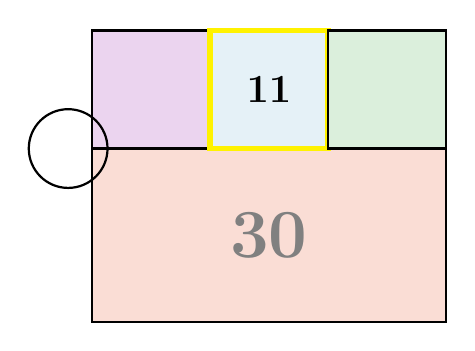
\begin{tikzpicture}[
    bar/.style={rectangle, draw, thick, minimum width=1.5cm, minimum height=1.5cm},
    mainbg/.style={rectangle, draw, thick, minimum width=4.5cm, minimum height=2.2cm, fill=p1!20, font=\Huge\bfseries\color{gray}}
]
    % Main HP Box
    \node[mainbg] (hp) at (2.25, 1.1) {30};
    
    % Top commander damage bars
    \node[bar, fill=p4!20] (b1) at (0.75, 2.95) {};
    % Highlighted Center Bar
    \node[bar, fill=p2!10, draw=yellow, line width=2pt, font=\Large\bfseries\color{black}] (b2) at (2.25, 2.95) {11}; 
    \node[bar, fill=p3!20] (b3) at (3.75, 2.95) {};
    
    % Knob attached to the left
    \node[circle, draw, thick, minimum size=1cm] (knob) at (-0.3, 2.2) {};
\end{tikzpicture}\\[0.5em]
\small\textit{Commander Mode Selection Highlight}
\end{center}
\vspace{1em}

\subsection{Land Play Tracker}
While in normal mode, hitting the knob button \textbf{once} toggles a "land played" status. This causes the main HP number and background to light up vividly. 

\begin{itemize}
    \item \textbf{Resetting:} Pressing the button again clears the status back to normal.
    \item \textbf{Interaction:} If another player hits their knob to mark their land play, it instantly resets your indicator and highlights theirs, ensuring the focus is strictly on the active player.
\end{itemize}

\vspace{1em}
\begin{center}
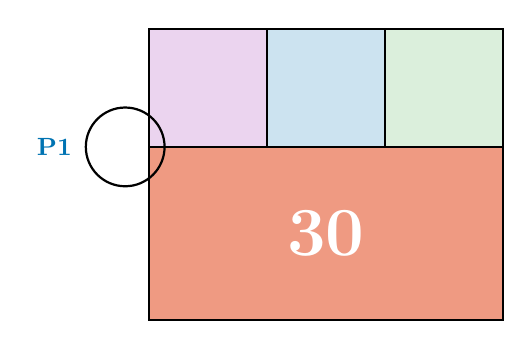
\begin{tikzpicture}[
    bar/.style={rectangle, draw, thick, minimum width=1.5cm, minimum height=1.5cm},
    hlbg/.style={rectangle, draw, thick, minimum width=4.5cm, minimum height=2.2cm, fill=p1!60, font=\Huge\bfseries\color{white}}
]
    % Highlighted Main HP Box
    \node[hlbg] (hp) at (2.25, 1.1) {30};
    
    % Top commander damage bars
    \node[bar, fill=p4!20] (b1) at (0.75, 2.95) {};
    \node[bar, fill=p2!20] (b2) at (2.25, 2.95) {};
    \node[bar, fill=p3!20] (b3) at (3.75, 2.95) {};
    
    % Knob attached to the left
    \node[circle, draw, thick, minimum size=1cm] (knob) at (-0.3, 2.2) {};
    
    % Player active indicator next to the knob
    \node[font=\small\bfseries, color=p2] at (-1.2, 2.2) {P1}; 
\end{tikzpicture}\\[0.5em]
\small\textit{Land Play Active Indicator}
\end{center}

\end{document}